\begin{frame}
  \frametitle{\problemtitle}
  \begin{block}{Problem}
    Given integers $n$, $a$ and $b$, find a permutation of building of heights $1$ to $n$ such that $a$ buildings can be seen from the left and $b$ buildings can be seen from the right, or say that none exists.
  \end{block}
  \begin{center}
    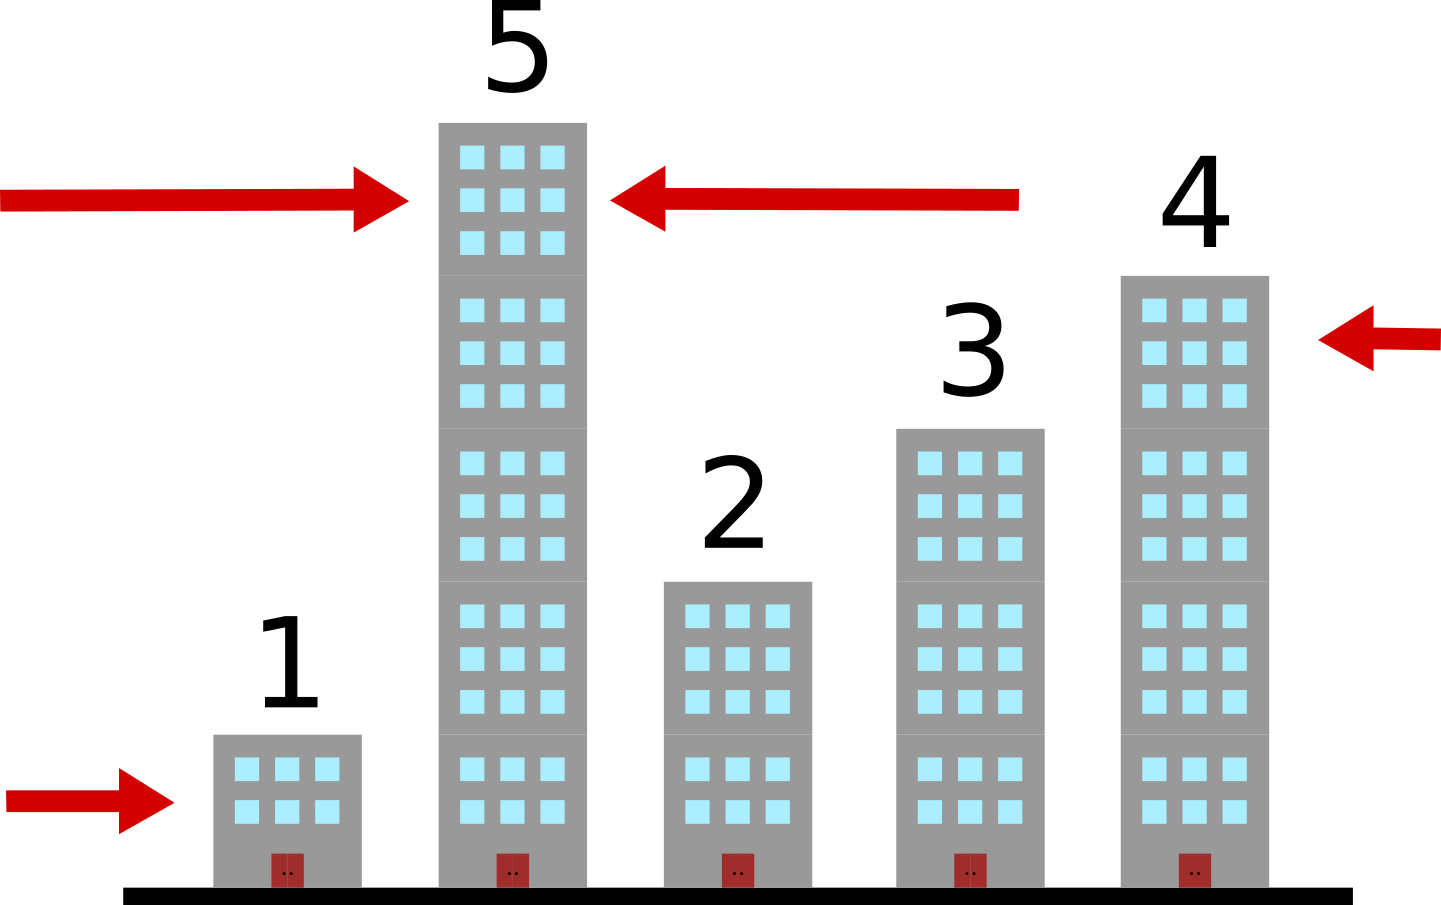
\includegraphics[width=0.6\textwidth]{sample1.png}
  \end{center}
\end{frame}
\begin{frame}
  \frametitle{\problemtitle}
  \begin{block}{Solution}
    \begin{itemize}
      \item There are two types of cases where no solution exists:
        \begin{itemize}
          \item Only building $n$ can be seen from both sides, so $a+b > n+1$ is impossible
          \item Building $n$ must always be next to a $1$ clue, so we cannot have $a = b = 1$
        \end{itemize}
      \item The following setup can be used in the general case:
        \begin{center}
          
\includegraphics[width=0.4\textwidth]{histogram.pdf}
        \end{center}
        \vspace{-3mm}
      \item If $a = 1$ or $b = 1$ you may need to reverse the middle part.
    \end{itemize}
  \end{block}
\end{frame}
